\section{Introduction}
\label{sec:intro}
%-------------------------------------------------------------------------
Semantic mapping targets the estimation of  the category to which each element in a scene belongs, along with a consistent geometric representation. Rich semantic representations in 3D are essential for advanced robotic applications.
Traditionally, semantic 3D reconstruction has relied on a closed-set approach in both offline~\cite{bao2011semantic,kundu2022panoptic} and online~\cite{mccormac2017semanticfusion,rosinol2020kimera} settings, including integrations into semantic Simultaneous Localization and Mapping (SLAM) systems~\cite{civera2011towards,zhu2024sni,li2024sgs}.
However, these methods are constrained by a predefined set of categories, which limits their flexibility and applicability in open-ended, real-world environments.
%Simultaneous Localization and Mapping (SLAM) refers to the online estimation of a platform's motion, along with a map of its surrounding environment, from the data streams of its onboard sensors~\cite{cadena2016past}. %While early SLAM research primarily targeted robotics, where it is seen as a fundamental step for autonomy~\cite{durrant2006simultaneous}, its widespread industrial adoption stemmed from augmented and virtual reality~\cite{klein2007parallel}.
%Visual SLAM research, however, has mainly focused on geometric models, sensor fusion, processing pipelines and optimizations~\cite{newcombe2011kinectfusion,whelan2015elasticfusion}, and much less and mostly recently on the crucial aspect of the scene representation~\cite{rosen2021advances}, that would further expand its potential for a wider array of tasks.

\begin{figure}[ht!]
    \centering
    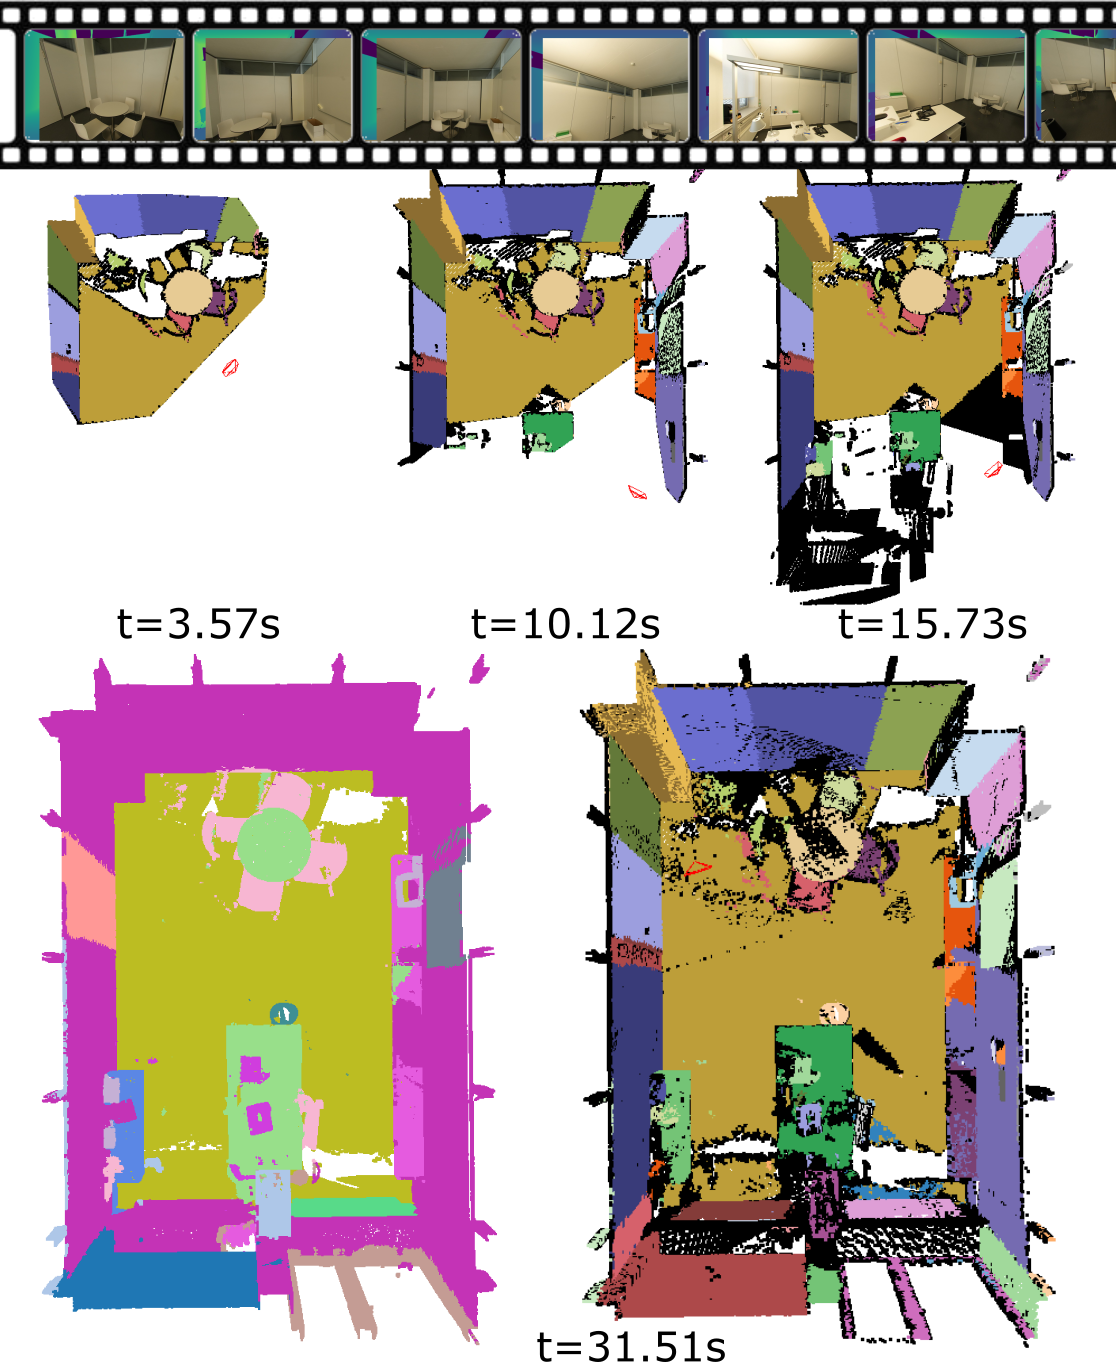
\includegraphics[width=0.9\linewidth]{figures/images/teaser.png}
    \resizebox{\linewidth}{!}
{
%\small
%\vspace{-28px}
\begin{tabular}{c}
\ColorMapCircle{spp_ceiling lamp}\,ceiling lamp
\ColorMapCircle{spp_bottle}\,bottle
\ColorMapCircle{spp_telephone}\,telephone 
\ColorMapCircle{spp_shelf}\,shelf
\small\ColorMapCircle{spp_wall}\,wall
\ColorMapCircle{spp_chair}\,chair
\ColorMapCircle{spp_door}\,door
\ColorMapCircle{spp_box}\,box\\
\small\ColorMapCircle{spp_whiteboard}\,whiteboard
\ColorMapCircle{spp_ceiling}\,ceiling
\ColorMapCircle{spp_cabinet}\,cabinet
\ColorMapCircle{spp_blinds}\,blinds 
\ColorMapCircle{spp_socket}\,socket 
\ColorMapCircle{spp_heater}\,heater
\ColorMapCircle{spp_table}\,table
\ColorMapCircle{spp_floor}\,floor
\ColorMapCircle{spp_window}\,window
\end{tabular}
}
%\vspace{-8px}
    \caption{\textbf{\ours mapping.} Given a RGB-D set of keyframes (\textbf{top}), our method successively reconstructs a 3D open-vocabulary representation of a scene over time (\textbf{middle}). 
    At any moment, both semantic labels (\textbf{bottom left}) as well as instance labels (\textbf{bottom right}) can be effectively recovered.
    }
    \label{fig:teaser}
\end{figure}
%Online semantic representations have taken various forms, e.g., object annotations in 3D point clouds~\cite{}, objects as high-level features~\cite{}, semantic segmentations of point cloud maps~\cite{} or implicit 3D representations~\cite{}.

Following the emergence of Contrastive Language-Image Pre-training (CLIP)~\cite{radford2021clip}, there has been a surge of interest in open-vocabulary 3D representations \cite{Peng2023OpenScene,takmaz2023openmask3d,nguyen2024open3dis}, including efforts in online mapping \cite{conceptfusion, gu2024conceptgraphs, yamazaki2024open}—though not yet in full SLAM systems.
While these recent approaches have shown strong performance, their dependence on offline processing or ground-truth camera poses for mapping significantly limits their applicability in robotics, augmented reality, and virtual reality scenarios.

In this paper, we present \ours, an \underline{O}pen-\underline{V}ocabulary \underline{O}nline mapping algorithm, which we integrate into two distinct visual SLAM pipelines. An example of our online reconstruction results is shown in \cref{fig:teaser}.
Our method processes RGB-D keyframes to generate 3D segments, each associated with a CLIP embedding.
These segments are initialized by back-projecting masks predicted by Segment Anything Model (SAM) 2.1~\cite{ravi2024sam2}, and are tracked over time by projecting them into 2D and matching against new masks.
Each 3D segment's CLIP descriptor is selected from the keyframe views with the best visibility.
Additionally, we introduce a novel model to extract per-instance CLIP descriptors directly from images, which are then assigned to the corresponding 3D masks.
{Our \clipours employs a neural network that learns per-dimension weighting to fuse CLIP descriptors of the same instance, while effectively generalizing to unseen classes and environments.}
Our pipeline not only operates online and supports loop-closure optimization, but also outperforms existing baselines in segmentation accuracy.